
%(BEGIN_QUESTION)
% Copyright 2013, Tony R. Kuphaldt, released under the Creative Commons Attribution License (v 1.0)
% This means you may do almost anything with this work of mine, so long as you give me proper credit

Write an equation to solve for the upstream pressure at this control valve, given the downstream pressure ($P_2$), $C_v$ factor, specific gravity ($G_f$) of the process liquid, and flow rate ($Q$):

$$\includegraphics[width=15.5cm]{i02746x01.eps}$$

\vskip 10pt

$P_1$ (formula) = 

\vskip 20pt

Then, solve for $P_1$ (in units of PSI) supposing the following conditions:

\begin{itemize}
\item{} $Q$ = 310 GPM
\item{} $G_f$ = 0.89
\item{} $P_2$ = 186 kPa
\item{} $C_v$ = 53
\end{itemize}

\vskip 10pt

\noindent
$P_1$ = \underbar{\hskip 50pt} PSI

\underbar{file i02746}
%(END_QUESTION)





%(BEGIN_ANSWER)

Half-credit for correct formula, half credit for correct numerical answer:

\vskip 10pt

$$P_1 = P_2 + G_f \left( {Q \over C_v} \right)^2$$

\vskip 10pt

\noindent
$P_1$ = 57.42 PSI

%(END_ANSWER)





%(BEGIN_NOTES)

{\bf This question is intended for exams only and not worksheets!}.

%(END_NOTES)


